\documentclass[aspectratio=169]{beamer}

% Theme and basics
\usetheme{Madrid}
\usecolortheme{default}
\usefonttheme{professionalfonts}
\setbeamertemplate{navigation symbols}{}

% Custom footline: short author and short title on all non-title slides
\setbeamertemplate{footline}{%
  \leavevmode
  \hbox{%
    \begin{beamercolorbox}[wd=\paperwidth,ht=2.5ex,dp=1ex,center]{author in head/foot}
      \usebeamerfont{author in head/foot}\insertshortauthor\,\textemdash\,\insertshorttitle
    \end{beamercolorbox}%
  }%
}

% Math and utilities
\usepackage{amsmath,amssymb,amsfonts}
\usepackage{bm}
\usepackage{graphicx}
\usepackage{subcaption}
\usepackage{booktabs}
\usepackage{tabularx}
\usepackage{arydshln}
\usepackage{array}
\usepackage{mathtools}
\usepackage{hyperref}
\usepackage{cleveref}
\usepackage{fontawesome5} % for question mark
%\usepackage[authoryear]{natbib}

% Absolute positioning for overlaying content on the title slide
\usepackage[absolute,overlay]{textpos}

\usepackage{environ}
\newcounter{aequation}
\NewEnviron{aequation}{\refstepcounter{aequation}$$\BODY\eqno{\text{(A\theaequation)}}$$}
\crefname{aequation}{assumption}{assumptions}
\creflabelformat{aequation}{(#2A#1#3)}


% Citations use the standard natbib formatting (as in the article)
\usepackage[style=authoryear, maxcitenames=1, maxbibnames=3, terseinits=true, uniquelist=false, natbib=true,]{biblatex}
\addbibresource{solo_slides.bib}
% Reuse article macros
\input{../conf_article/math_commands.tex}

\newcommand{\norm}[1]{\lVert #1\rVert}
\newcommand{\abs}[1]{\lvert #1 \rvert}

% \epsilon is predefined; override to use \varepsilon
\renewcommand{\epsilon}{\varepsilon}
\newcommand{\Rmn}{\R^{m\times n}}
\newcommand{\cB}{\mathcal{B}}
\newcommand{\cD}{\mathcal{D}}
\newcommand{\cN}{\mathcal{N}}
\newcommand{\cO}{\mathcal{O}}
\newcommand{\cS}{\mathcal{S}}
\newcommand{\Ed}[2]{\mathbb{E}_{#1}\left[#2\right]}
\usepackage{mathtools}
\DeclarePairedDelimiter{\sqne}{\|}{\|_2^2}
%\DeclarePairedDelimiter{\norme}{\|}{\|_2}
\DeclarePairedDelimiter{\normf}{\|}{\|_\mathrm{F}}
\DeclarePairedDelimiter{\normkfk}{\|}{\|_\mathrm{KF-k}}
\DeclarePairedDelimiter{\normfstar}{\|}{\|_\mathrm{F*}}
\DeclarePairedDelimiter{\normftwo}{\|}{\|_\mathrm{F2}}
\DeclarePairedDelimiter{\sqns}{\|}{\|_{\mathrm{op}}^2}
\DeclarePairedDelimiter{\norms}{\|}{\|_{\mathrm{op}}}
\DeclarePairedDelimiter{\sqnn}{\|}{\|_{\mathrm{nuc}}^2}
\DeclarePairedDelimiter{\sqnf}{\|}{\|_{\mathrm{F}}^2}
\DeclarePairedDelimiter{\normn}{\|}{\|_{\mathrm{nuc}}}
\DeclarePairedDelimiter{\normfkfk}{\|}{\|_{\mathrm{F-KF-k}}}
\def\<#1,#2>{\langle #1,#2\rangle}
\DeclarePairedDelimiter{\dotprod}{\langle}{\rangle}

\DeclareMathOperator{\tr}{tr}
\DeclareMathOperator{\diag}{diag}

% Graphics from the article repo
\graphicspath{{../article_final/figs/}}

% Title
\title[The Ky Fan Norms and Beyond]{The Ky Fan Norms and Beyond: Dual Norms and Combinations for Matrix Optimization}
\author[A. Kravatskiy]{%
  Alexey Kravatskiy\\[0.3em]
}
\institute[]{%
MIPT \hspace{1em}%
}
\date{\today}

\begin{document}

%-------------------------------------------------------------------------------------
\begin{frame}[plain]
  \titlepage
  % Right-side figure on the title slide
  \begin{textblock*}{0.2\paperwidth}(0.75\paperwidth,0.6\paperheight)
    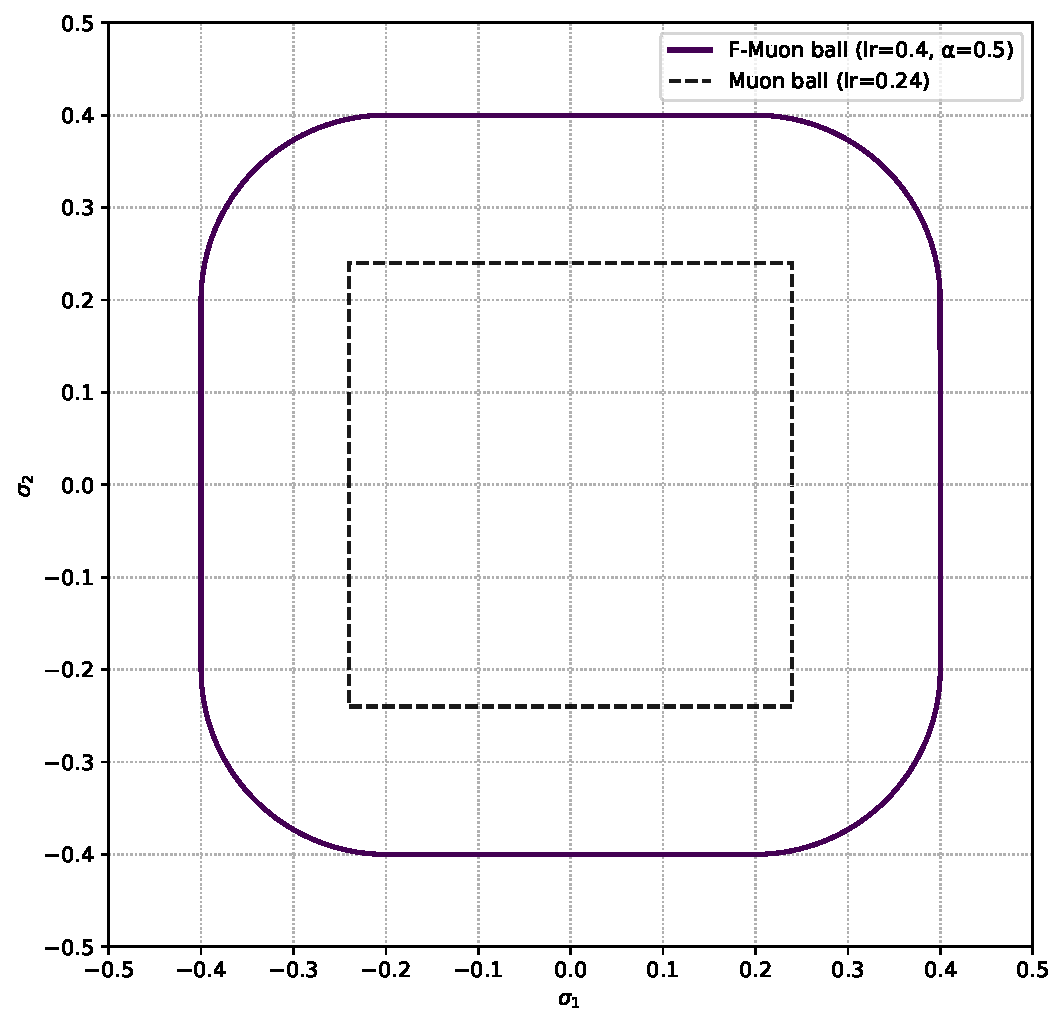
\includegraphics[width=\linewidth]{norms/fstardual_cifar.pdf}
  \end{textblock*}
  \begin{textblock*}{0.22\paperwidth}(0.05\paperwidth,0.55\paperheight)
    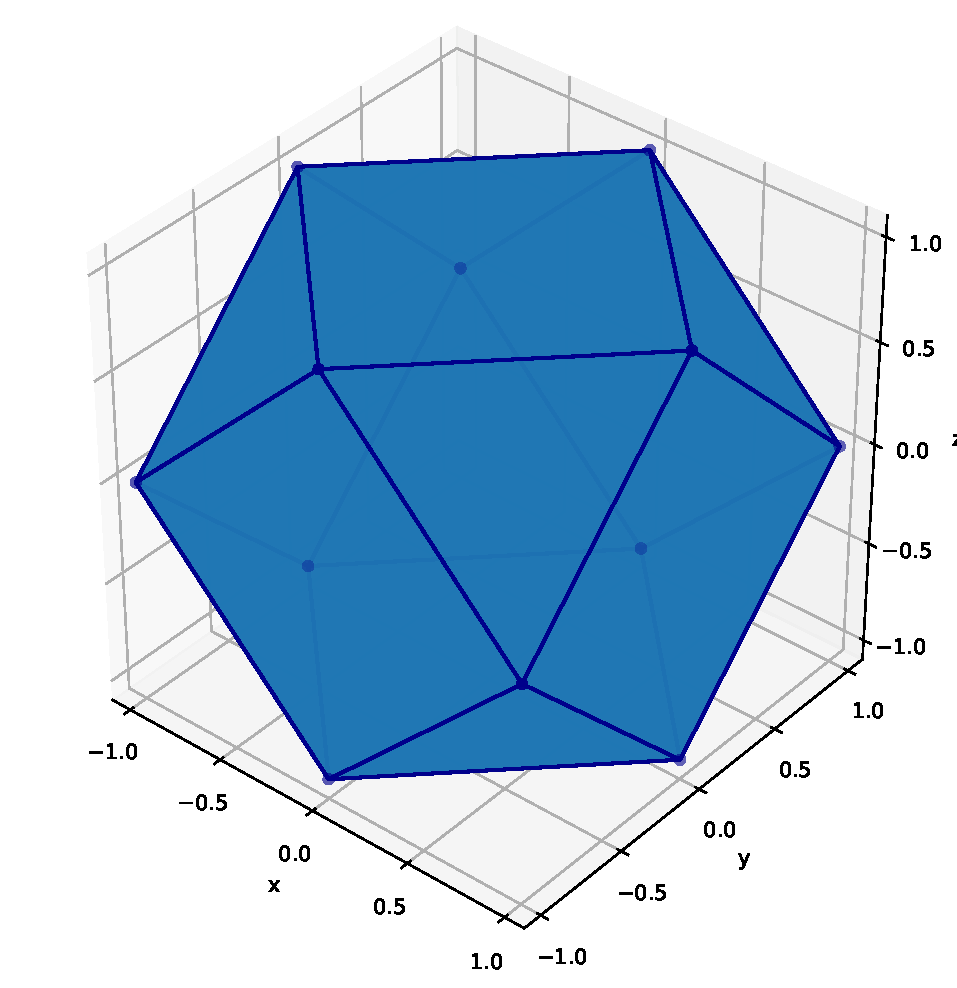
\includegraphics[width=\linewidth]{norms/KyFanDual.pdf}
  \end{textblock*}
\end{frame}
%-------------------------------------------------------------------------------------
\begin{frame}{Moving beyond the spectral norm and Muon}
    \begin{block}{F-Fanions: Muon, Neon, NSGD, Dion without EF, and so much more}
        From $\norms{\cdot}$ and Muon:
        $$\mX^{t+1} = \mX^{t} - \eta U V^\top$$
        To $\normkfk{\cdot}^\dagger$ and a general F-Fanion:
        $$\mX^{t+1} = \mX^{t} - \eta \left(\alpha \sum_{i=1}^k{u_i v_i^\top} + (1-\alpha)\frac{\mM^t}{\normf{\mM^t}}\right), \alpha \in [0,1]$$
        To $\norm{\cdot}^\dagger_{\mathrm{C^\dagger-KF-k}}$ and a general S-Fanion:
        $$\mX^{t+1} = \mX^{t} - \gamma_t \left(\alpha \sum_{i = 1}^k \vu_i \vv_i^\top + (1-\alpha)\eta\sign(\mM^t)\right)\, \alpha \in [0,1], \eta > 0$$
    \end{block}
      
\end{frame}
%-------------------------------------------------------------------------------------
\begin{frame}{Linear Minimization Oracle (LMO)}
% after omitting gamma_k, we obtain:
Let us equip $\Rmn$ with a norm $\norm{\cdot}$. Its dual is $\norm{\mX}^\dagger = \sup_{\norm{\mX'}\leq 1} \<\mX,\mX'>$. $\<\cdot, \cdot>$ is the Frobenius product.
\vspace{0.4em}

LMO leads to the update
$$\mX^{t+1} = \mX^{t} - \eta \arg\max_{\mX \in \cB_1} \<\mM^t, \mX> = \mX^{t} - \eta \{\Delta \in \cB_1 \mid \<\mM^t, \Delta> = \norm{\mM^t}^\dagger\}$$

\vspace{0.4em}

\textbf{Recipe}: It means we seek $\Delta$ from the 1-norm ball that delivers $\<\mM^t, \Delta> = \norm{\mM^t}^\dagger$
\vspace{0.4em}

We will often utilize the SVD of $\mM^t$: $\mM^t = \mU \Sigma \mV^\top$.
\end{frame}
\begin{frame}{Of Matrix and Vector Algorithms}
    %\centering
    %\def\arraystretch{1.1}
    \footnotesize
    \begin{table}
    \caption{lmo optimizers in Schatten $S_p$ norms and in $l_p$ norms.}
    \label{tbl:mat_vs_vec_lmo}
    \begin{tabularx}{\linewidth}{|>{\raggedright\arraybackslash}X|c|c|c|}
    \hline
    Method & lmo constraint set $\mathcal D$ & lmo & Reference \\
    \hline\hline
    Normalized SGD & $l_2$-ball, $S_2$-ball & $-\eta \tfrac{g}{\norm{g}_2} = -\eta \tfrac{g}{\norm{g}_F}$ & \citep{hazan2015beyond} \\
    Momentum Normalized SGD & Ball in $l_2$, or Ball in $S_2$ & $-\eta \tfrac{g}{\norm{g}_2} = -\eta\tfrac{g}{\norm{g}_F}$ & \citep{cutkosky2020momentum}\\
    \hline
    SignSGD & Ball in Max-norm $l_\infty$ & $-\eta \sign(g)$ & \citep[Thm. 1]{bernstein2018signsgd} \\
    Signum  & Ball in Max-norm $l_\infty$ & $-\eta \sign(g)$ & \citep[Thm. 3]{bernstein2018signsgd} \\
    \hdashline
    Muon & Ball in Spectral $S_\infty$ & $-\eta UV^\top$ & \citep{jordan2024muon} \\
    \hline
    Gauss-Southwell Coordinate Descent & Ball in $l_1$ & $-\eta \sum_{i \in \argmax|g_i^t|} \sign(g_i^t)e_i$ & \citep[p.19]{shi2016primer}\\
    \hdashline 
    Neon & Ball in Nuclear $S_1$ & $-\eta u_1 v_1^\top$ & \citep{kravatskiy2025fanions} \\
    $\nu$SAM & & & \citep{pethick2025sam} \\
    \hline
    \end{tabularx}
    \end{table}
\end{frame}
\begin{frame}{The rank gap problem}
Schatten $p$-norms $\norm{\mM^t}_{S_p} = \left(\sum_{i=1}^{\min(m, n)}\sigma_i^p\right)^{1/p}\,$
  produce the update
 \[
 \mX^{t+1} = \mX^t - \gamma_t \mU \frac{\diag\left(\sigma_1^{q-1},\dots, \sigma_{\min(m,n)}^{q-1}\right)}{\left(\sum_{i=1}^{\min(m,n)}{\sigma_i^q}\right)^{\frac{q-1}{q}}}\mV^\top
 \]
 where $p$ and $q$ satisfy $p^{-1} + q^{-1} = 1$ \citep{cesista2025schattenp}.

 \vspace{0.5em}
 Ky Fan $k$-norms $\normkfk{\mM^t}= \sum_{i=1}^{k}\sigma_i\,$ produce either
 \[
 \mX^{t+1} = \mX^{t} - \gamma_t \vu_1 \vv_1^\top\text{ or }\mX^{t+1} = \mX^{t} - \frac{\gamma_t}{k}\mU \mV^\top\,,
 \]
that is either Neon or Muon \citep{kravatskiy2025fanions}.

\vspace{0.5em}

Thus, the updates are either one-rank or full-rank.

\end{frame}

%----------------------------------------------------------------------------------------------------------
\begin{frame}{Ky Fan $k$-rank $\normkfk{\mM^k}^\dagger$ and Fanions}

\begin{block}{Deriving Fanions by Recipe} $\normkfk{\mM^t}^{\dagger\dagger} = \normkfk{\mM^t}$, and $\Delta = \sum_{i=1}^k{u_i v_i^\top}$ with $\normkfk{\Delta}^\dagger = \max\{\frac{1}{k} \normn{\Delta}, \norms{\Delta}\} = \max\{\frac{1}{k} k, 1\} = 1$ delivers it:
    $$\<\mM^t, \Delta> =\<\mU \mSigma \mV^\top, \sum_{i=1}^{k} u_i v_i^\top> = \sum_{i,j=1}^{r, k}\<u_i \sigma_i v_i^\top, u_j v_j^\top> = \sum_{i=1}^{k}\sigma_i = \normkfk{\mM^t}$$
    
    Hence,
    $$\mX^{t+1} = \mX^{t} - \eta \sum_{i=1}^{k} u_i v_i^\top$$
    \end{block}
\end{frame}
%-----------------------------------------------------------------------------------------------------------
\begin{frame}{Geometric point of view: Ky Fan norms}
  \centering
  \begin{minipage}{0.46\textwidth}
      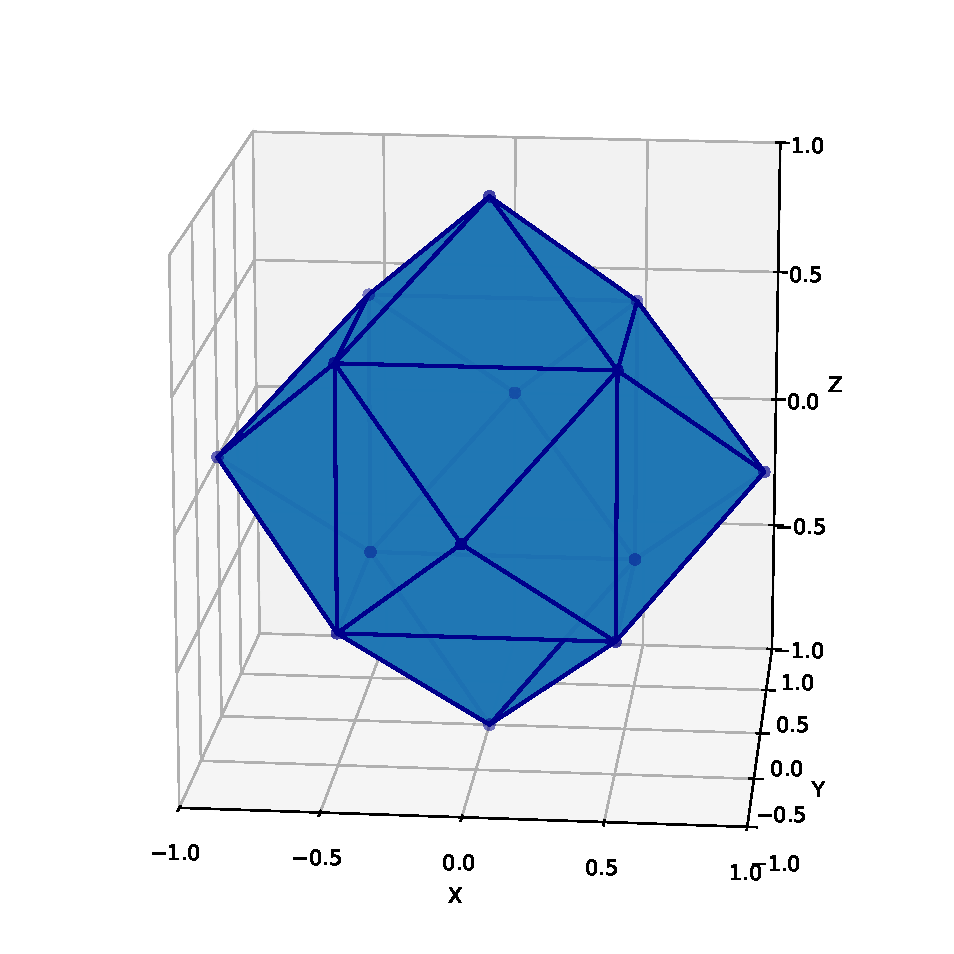
\includegraphics[height=0.75\textheight,keepaspectratio]{norms/KyFan.pdf}
  \end{minipage}\hfill
  \begin{minipage}{0.46\textwidth}
      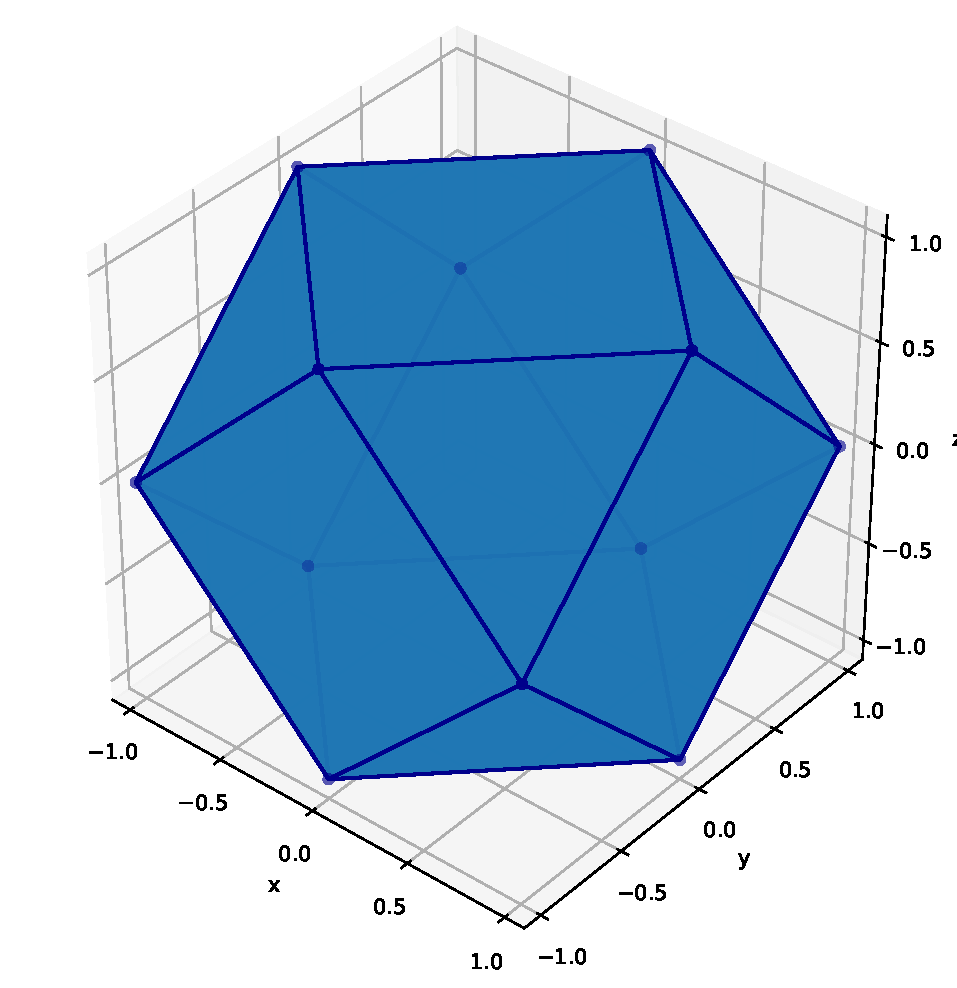
\includegraphics[height=0.75\textheight,keepaspectratio]{norms/KyFanDual.pdf}
  \end{minipage}
  
  \vspace{0.3em}
  \footnotesize Ky Fan rank-2 ball and its dual in a 3D singular-value space
  \end{frame}
%--------------------------------------------------------------------------------------------------------------
%--------------------------------------------------------------------------------------------------------------
\begin{frame}{Balls of duals to convex combinations of norms}
  \begin{lemma}\label{lemma:dual_to_conv_comb}
    Let $\norm{\cdot}_{(1)},\dots,\norm{\cdot}_{(n)}$ be norms on a finite-dimensional Euclidean space, and let $\alpha_1,\dots,\alpha_n$ be non-negative reals. Define
    \[
      \norm{\cdot} := \sum_{i = 1}^n \alpha_i \norm{\cdot}_{(i)}\,.
    \]
    Then the dual unit ball of $\norm{\cdot}$ satisfies
    \[
      \cB_{\norm{\cdot}^\dagger}
      = \sum_{i = 1}^n \alpha_i \cB_{\norm{\cdot}_{(i)}^\dagger}\,,
    \]
    where $\sum$ denotes the Minkowski sum and $\cB_{\norm{\cdot}_{(i)}^\dagger}$ is the unit ball of the dual norm $\norm{\cdot}_{(i)}^\dagger$.
  \end{lemma}
  
    
\end{frame}
%--------------------------------------------------------------------------------------------------------------
\begin{frame}{Conic combination of LMO algorithms is an LMO algorithm}
\begin{corollary}\label{corollary:lin_comb_alg}
  Let there be a finite family of LMO-based algorithms indexed by $i = 1,\dots,n$, where the $\mX^{t + 1}$ update in the $i$-th algorithm is defined by
  \[
  \mX^{t + 1} - \mX^{t} = \gamma_t \mathrm{LMO}_{i}(\mM^{t})\,,
  \]
  and $\mathrm{LMO}_i$ corresponds to the unit ball of norm $\norm{\cdot}_i$. For arbitrary non-negative $\alpha_1,\dots,\alpha_n$, the algorithm with the update given by
  \[
  \mX^{t + 1} - \mX^{t} = \gamma_t \sum_{i = 1}^n \alpha_i \mathrm{LMO}_{\norm{\cdot}_{(i)}}(\mM^t)
  \]
  is an LMO-algorithm itself, with LMO corresponding to the unit ball of the norm $\norm{\cdot}$ dual to the norm given by $\sum_{i = 1}^n \alpha_i \norm{\cdot}_{(i)}^\dagger$.
\end{corollary}
\end{frame}
%-----------------------------------------------------------------------------------------------------------
\begin{frame}{$\normfkfk{\mM^k}^\dagger$ and F-Fanions}

    \begin{block}{Deriving F-Fanions by Recipe}
    $\normfkfk{\mM^t}^{\dagger\dagger} = \normfkfk{\mM^t}$, and $\Delta = \alpha\sum_{i=1}^k{u_i v_i^\top} + (1-\alpha)\frac{\mM^k}{\normf{\mM^k}}$ delivers it:
\begin{enumerate}
    \item $\normfkfk{\Delta}^\dagger \leq 1$ because $\sum_{i=1}^k{u_i v_i^\top}$ lies in $B_{\normkfk{\cdot}}$ and $\frac{\mM^k}{\normf{\mM^k}}$ lies in $B_{\normf{\cdot}}$, so $\Delta$ lies in the Minkowski sum
    \item $\<\mM^t, \Delta> =\alpha \<\mU \mSigma \mV^\top, \sum_{i=1}^{k} u_i v_i^\top> + (1-\alpha)\<\mM^t, \frac{\mM^t}{\normf{\mM^t}}> = \alpha \sum_{i=1}^{k}\sigma_i + (1-\alpha) \normf{\mM^t}= \normfkfk{\mM^t}$
\end{enumerate}
\vspace{1em}

        Hence,
        $$\mX^{t+1} = \mX^{t} - \eta \Big(\alpha\sum_{i=1}^{k} u_i v_i^\top + (1-\alpha)\frac{\mM^t}{\normf{\mM^t}}\Big)$$
        \end{block}
\end{frame}
%----------------------------------------
\begin{frame}{A smooth convex problem for a matrix}
  \begin{columns}[T,totalwidth=\textwidth]
    \begin{column}{0.48\textwidth}
      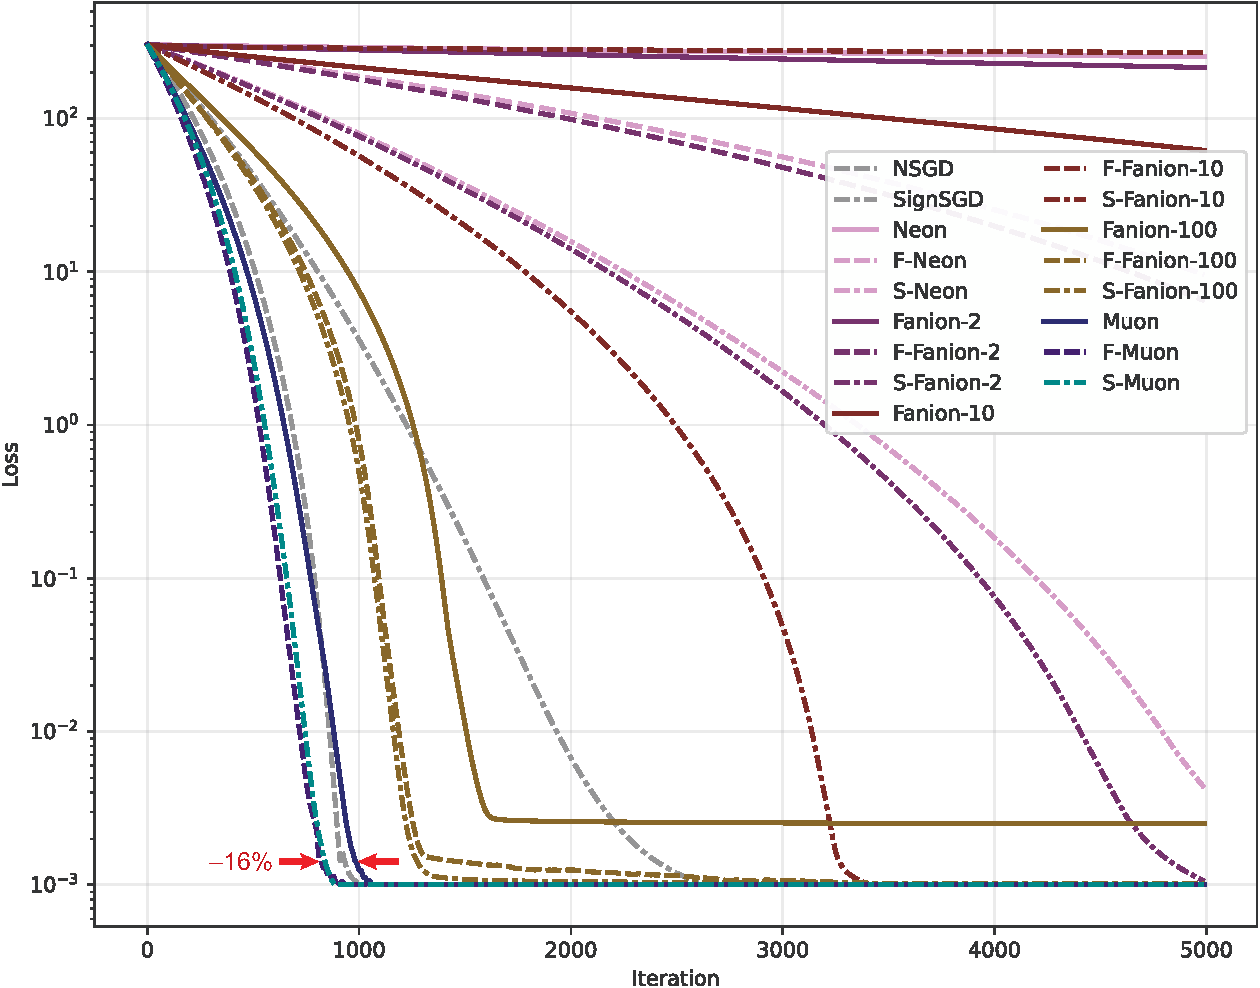
\includegraphics[width=\linewidth]{simple_lls/loss_long_run_16_increase.pdf}
      \centering
      \scriptsize Loss vs iteration
    \end{column}
    \begin{column}{0.48\textwidth}
      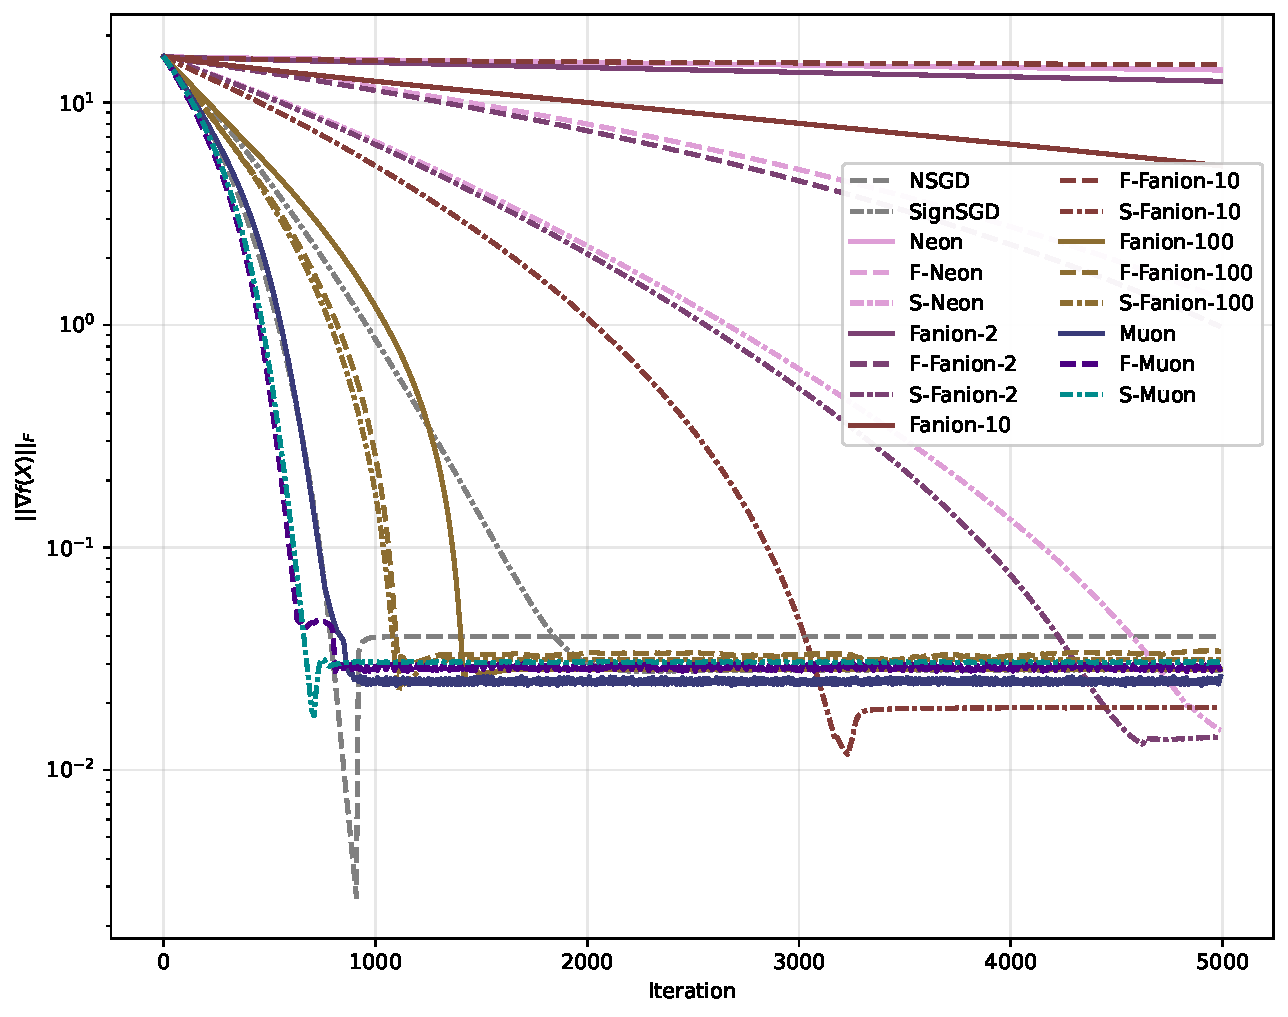
\includegraphics[width=\linewidth]{simple_lls/gradient_frobenius_norm_vs_iteration_long_run.pdf}
      \centering
      \scriptsize Frobenius norm of the gradient vs iteration
    \end{column}
  \end{columns}
  \vspace{0.3em}
  \centering
  \footnotesize $F(\mX) = \frac{1}{2}\normf{\mM^{1/2}\mX\mN^{1/2}}^2 \to \min_{\mX \in \R^{500\times 500}}\,$, $\lambda(\mM), \lambda(\mN) \sim U[0,1]$, $\mX^0_{ij} \sim \cN(0,1)$
\end{frame}

%---------------------------------------
\begin{frame}{F-Muon on CIFAR-10 airbench}
    \begin{columns}[T,totalwidth=\textwidth]
      \begin{column}{0.48\textwidth}
        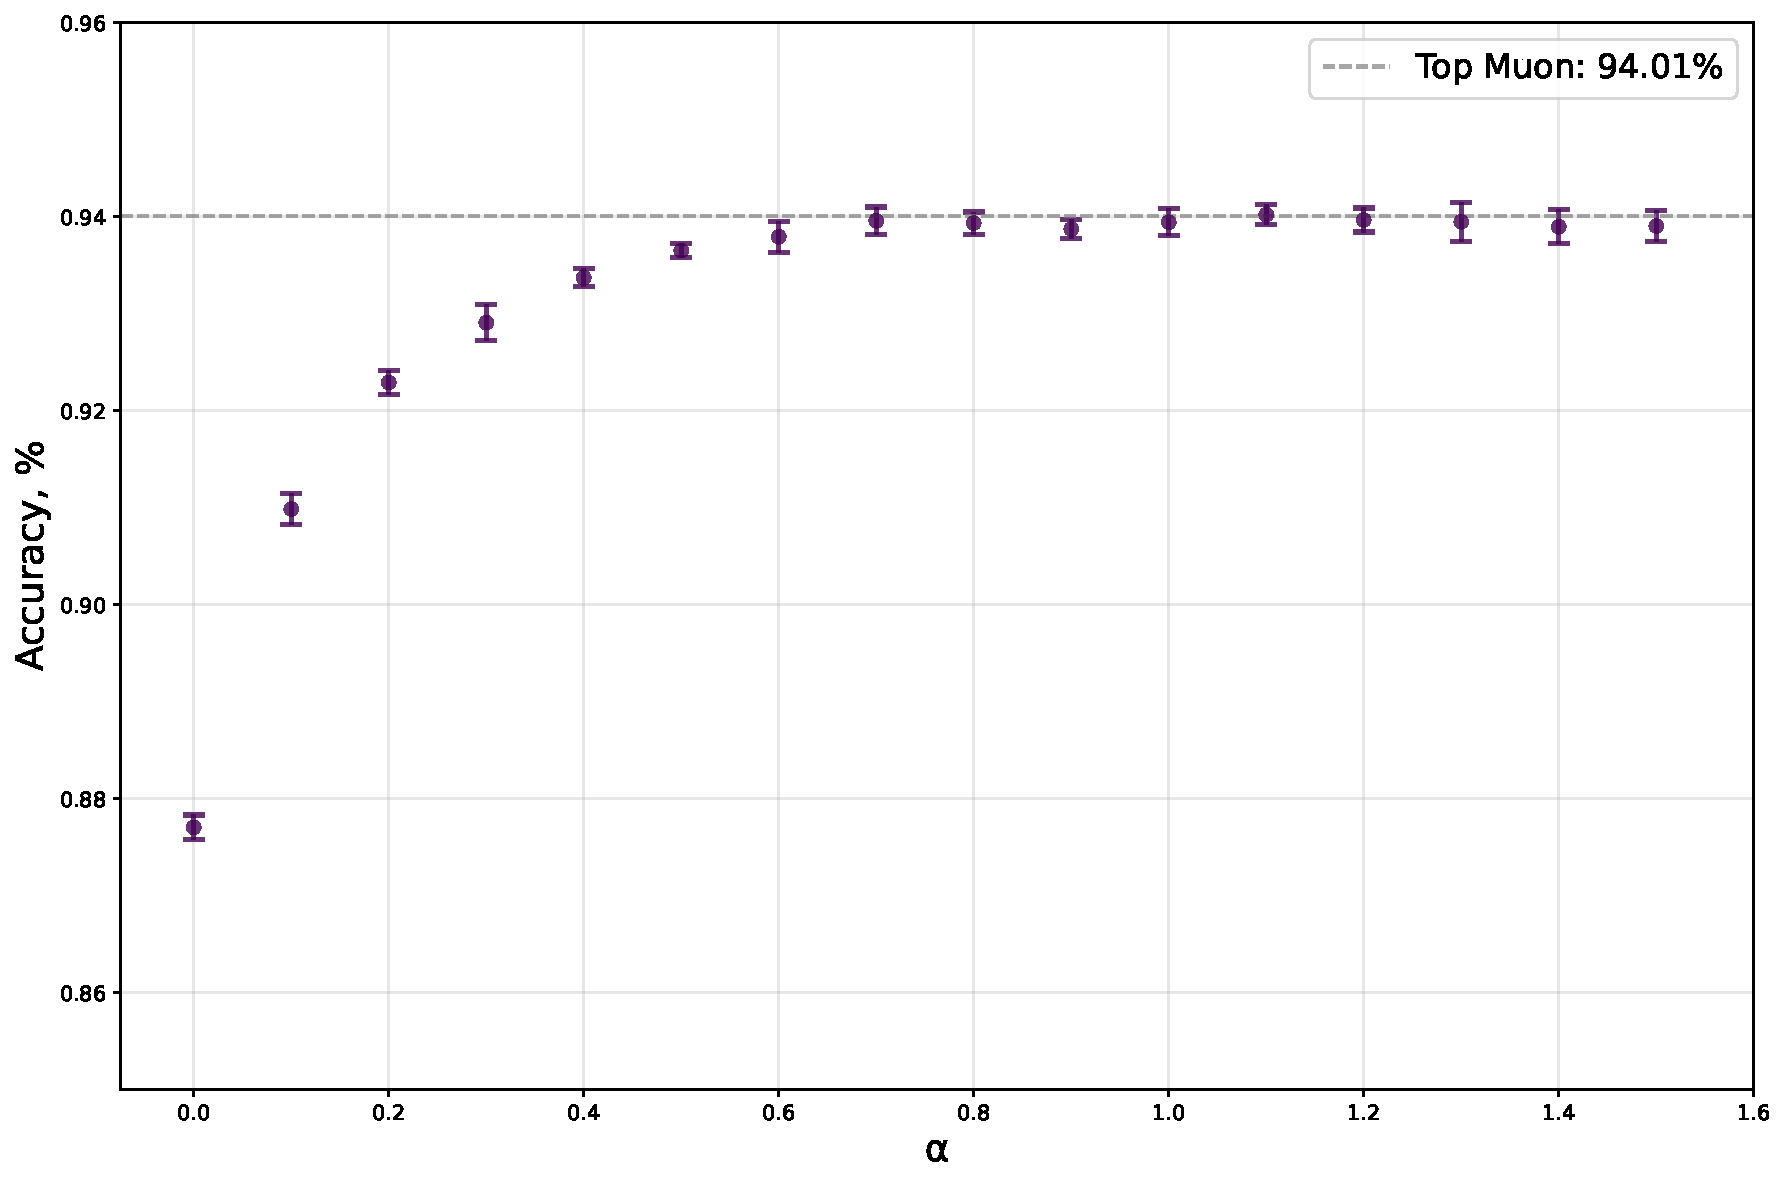
\includegraphics[width=\linewidth]{muon_tuned_diff_alpha.pdf}
        \centering
        \scriptsize With params tuned for Muon, as in \citep{cifar2023airbench}
      \end{column}
      \begin{column}{0.48\textwidth}
        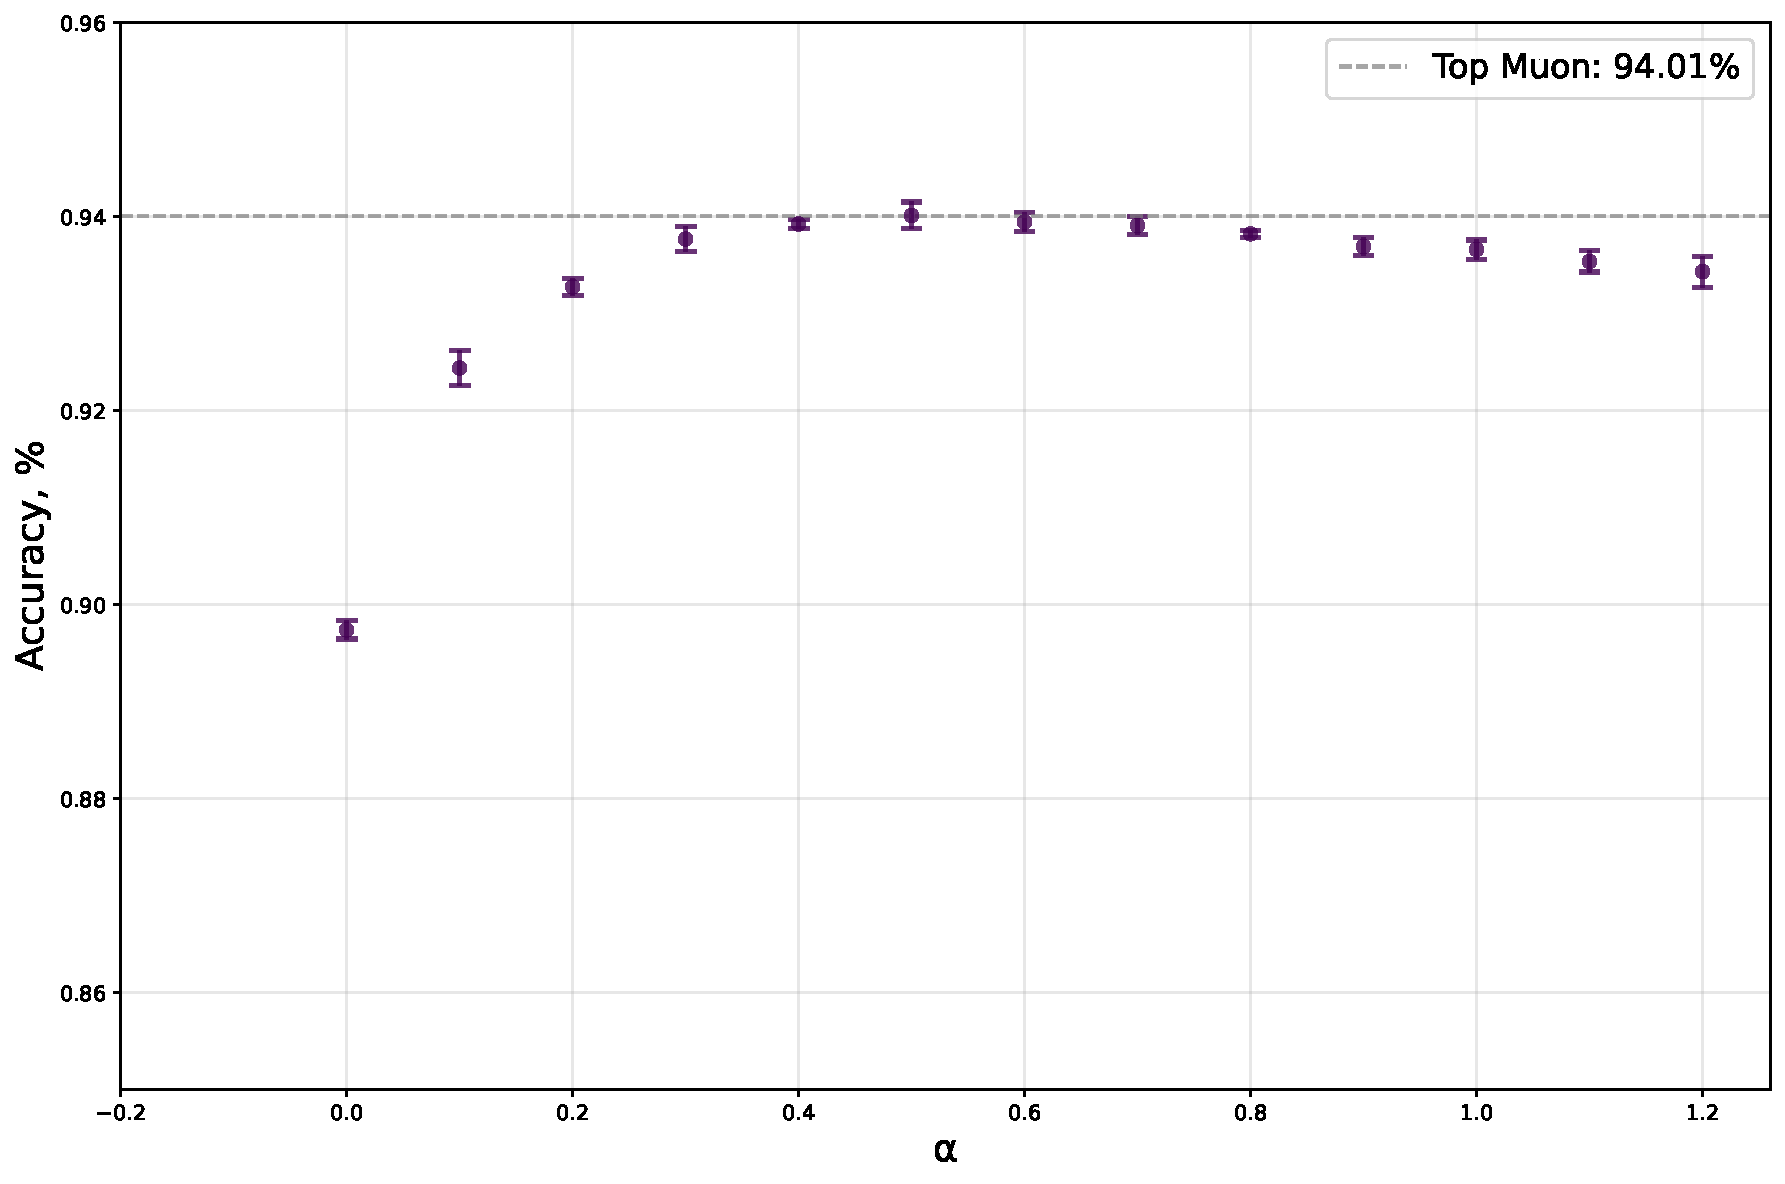
\includegraphics[width=\linewidth]{fmuon_tuned_diff_alpha.pdf}
        \centering
        \scriptsize With params tuned for $\alpha=0.5$ F-Muon
      \end{column}
    \end{columns}
    \vspace{0.6em}
    \centering

    \footnotesize F-Muon with \(\alpha = 0.5\) matches Muon after tuning

    \faExclamationCircle \space F-Fanion with $\alpha > 1$ is not an LMO algorithm
  \end{frame}

%----------------------------------------
\begin{frame}{LMO balls on CIFAR-10}
  \begin{figure}[t]
    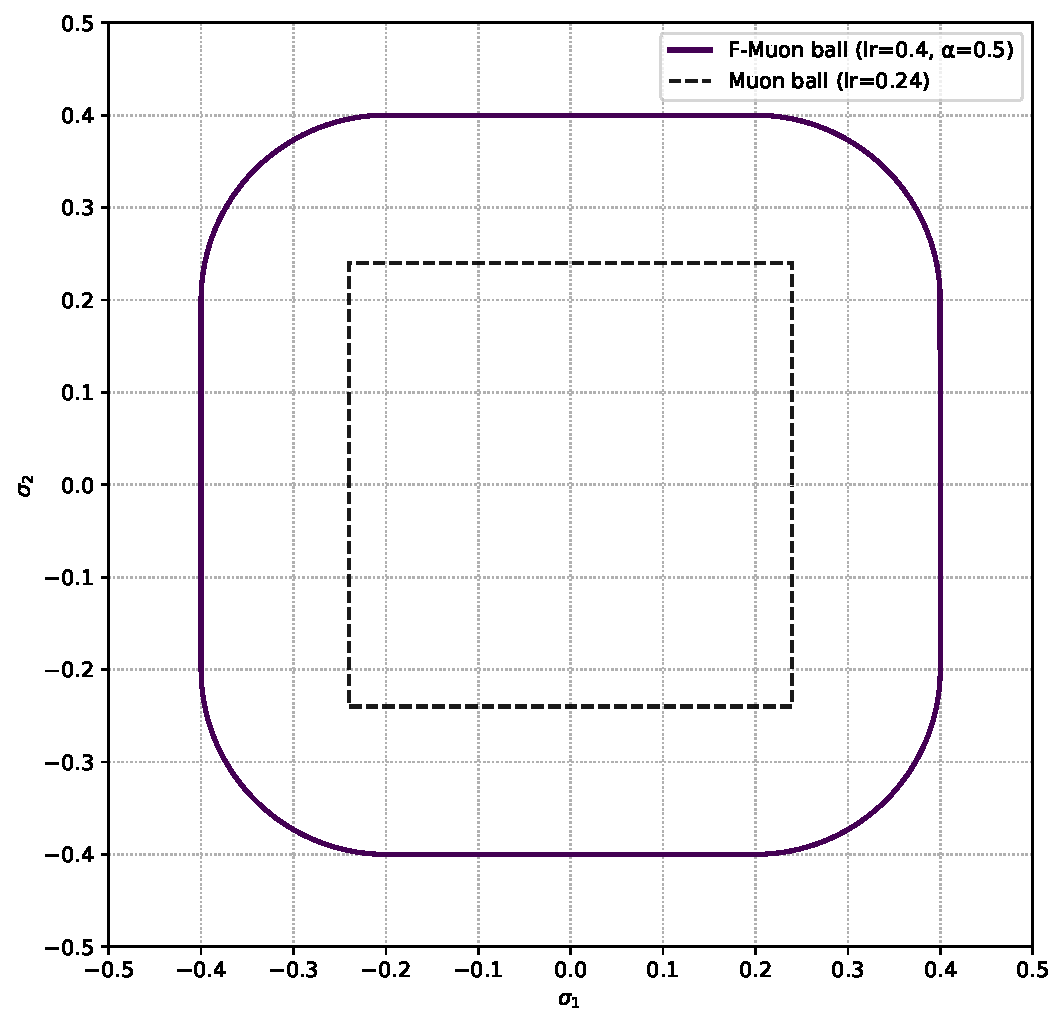
\includegraphics[height=0.7\textheight]{norms/fstardual_cifar.pdf}
    \centering

    \footnotesize LMO balls for the learning rates from the experiments

  \end{figure}
\end{frame}
%-----------------------------------------
\begin{frame}{NanoGPT and GPT-2 Medium}
  \begin{columns}[T,totalwidth=\textwidth]
    \begin{column}{0.48\textwidth}
      
\includegraphics[width=\linewidth]{nanogpt/nano/val_loss_vs_step.pdf}
      \centering
      \scriptsize NanoGPT
    \end{column}
    \begin{column}{0.48\textwidth}
      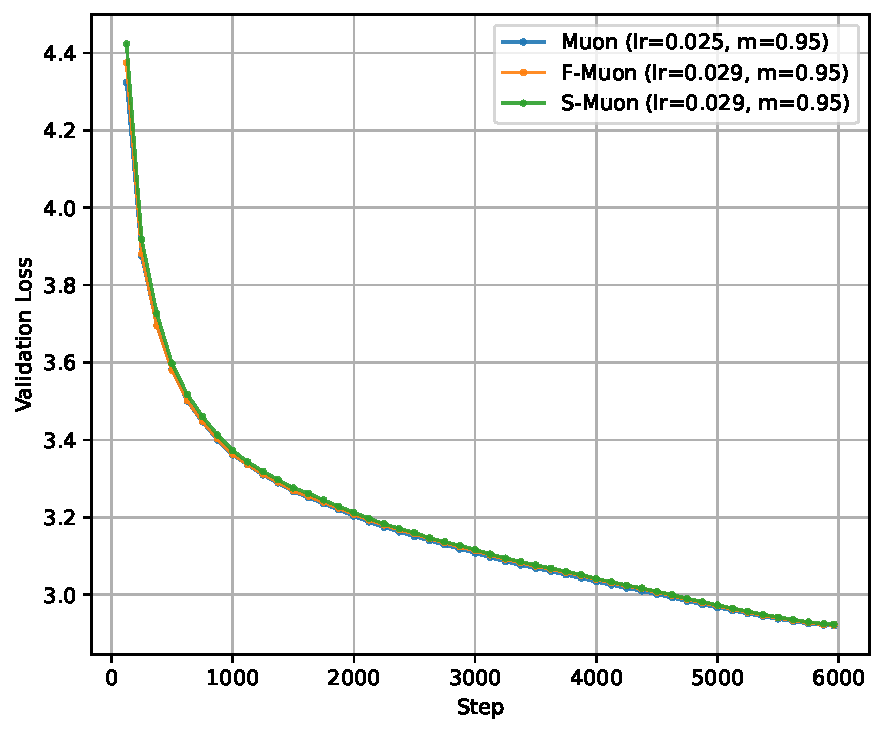
\includegraphics[width=\linewidth]{nanogpt/medium/val_loss_vs_step.pdf}
      \centering
      \scriptsize GPT-2 Medium
    \end{column}
  \end{columns}
  \vspace{0.3em}
  \centering
\end{frame}
%----------------------------------------
\begin{frame}{Conclusion}
  \begin{itemize}
    \item Muon, $\nu$-SAM, and Dion withour error feedback are Fanions
    \item A combination of LMO algorithms is an LMO algorithm
    \item F-Muon and S-Muon are on par with Muon
  \end{itemize}

  \vspace{2em}
  \textbf{For the future}: Estimating $(L_0, L_1)$ smoothness for new norms, as in \citep{riabinin2025gluon}
\end{frame}

%----------------------------------------
\begin{frame}[allowframebreaks]{References}
  % Match article's bibliography style and entries
  \printbibliography
  %\bibliographystyle{../conf_article/icomp2024_conference}
  %\bibliography{../conf_article/icomp2024_conference}
\end{frame}

\end{document}


